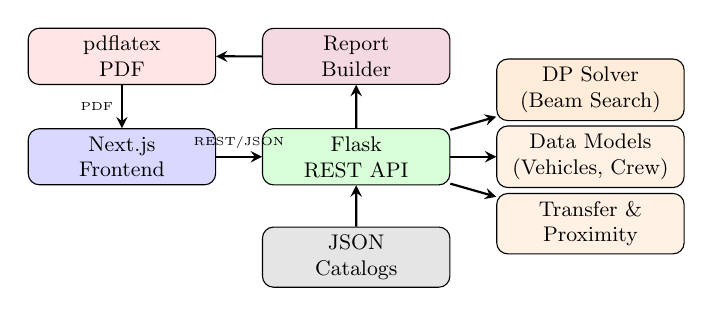
\begin{tikzpicture}[
  box/.style={draw, rounded corners, minimum width=2.8cm,
              minimum height=0.7cm, align=center, font=\small},
  arr/.style={->, >=stealth, thick},
  scale=0.85, transform shape
]
% Frontend box
\node[box, fill=blue!15] (fe) at (0,0) {Next.js\\Frontend};
% API box
\node[box, fill=green!15] (api) at (3.5,0) {Flask\\REST API};
% Solver
\node[box, fill=orange!15] (solver) at (7,1) {DP Solver\\(Beam Search)};
% Models
\node[box, fill=orange!10] (models) at (7,0) {Data Models\\(Vehicles, Crew)};
% Transfer
\node[box, fill=orange!10] (transfer) at (7,-1) {Transfer \&\\Proximity};
% Data
\node[box, fill=gray!20] (data) at (3.5,-1.5) {JSON\\Catalogs};
% Report
\node[box, fill=purple!15] (report) at (3.5,1.5) {Report\\Builder};
% pdflatex
\node[box, fill=red!10] (pdf) at (0,1.5) {pdflatex\\PDF};

\draw[arr] (fe) -- node[above,font=\tiny]{REST/JSON} (api);
\draw[arr] (api) -- (solver);
\draw[arr] (api) -- (models);
\draw[arr] (api) -- (transfer);
\draw[arr] (data) -- (api);
\draw[arr] (api) -- (report);
\draw[arr] (report) -- (pdf);
\draw[arr] (pdf) -- node[left,font=\tiny]{PDF} (fe);
\end{tikzpicture}
